\documentclass{article}
\usepackage[utf8]{inputenc}
\usepackage{subcaption}
\usepackage{amsmath}
\usepackage{amssymb}
\usepackage{hyperref}
\usepackage{titlesec}
\usepackage{xcolor}
\usepackage{fancyhdr}
\usepackage{graphicx}
\usepackage{tcolorbox}
\usepackage{multirow}
\usepackage[rightcaption]{sidecap}
\usepackage{verbatim}
\usepackage[backend=bibtex]{biblatex}
\usepackage{blindtext}
\usepackage{multicol}
\usepackage [ a4paper , top = 0.8 in, hmargin = 0.8 in , bottom =0.8 in ] { geometry }
\hypersetup{
    colorlinks=true,
    linkcolor=blue,
    filecolor=magenta,      
    urlcolor=cyan,
}
\setlength\parindent{0pt}
\usepackage{enumitem}

\bibliography{bibliography}
\fancyhead[L]{CS349}
\fancyhead[R]{Project Submission Stage 1}
\fancyfoot[C]{Page \thepage}

\DeclareMathOperator*{\maxi}{max}
\DeclareMathOperator*{\mini}{min}

\graphicspath{{images/}}

\begin{document}

\title{\large{CS349: Project Submission Stage 1} \\ \Huge \textbf{XData Extensions}}
\date{}
\author{Satyankar Chandra (22B0967) \\
Ayan Tanwar (22B0931) \\
Gourish Garg (22B0915) \\
Harsh Kumar (22B0973)}
\pagestyle{fancy}

\maketitle

\section{Project Overview}

\textbf{Aim:} Extend XData to support in-browse postgresql execution using \href{https://pglite.dev/}{pglite.dev}. Make sure everything runs from local resources so it can be run for exams without external internet. This allows each user to run in their own database without accessing any central database. The next step is to extend XData system to run the queries in browser rather than on a backend database.

\section{Project Proposal}

In our initial project proposal, we aimed to extend the XData system and implement the following features:
\begin{itemize}
    \item Query Profiling and Runtime Analysis
    \item Evaluation Plans and Query Optimization
    \item Client Side Autograding
    \item Support for Concurrent Queries
    \item Adding Constraints to Queries
\end{itemize}

Our team has been working on all of these features in parallel. We have made significant progress on the first two features, and we are currently working on the third and fourth features. The fifth feature is still in the planning stage.

\section{Current Progress}

Below is the current status of our project for each of the features:

\subsection{Query Profiling and Runtime Analysis}

We have built the foundation for profiling SQL queries by breaking them down into their smallest executable subqueries. Using a JavaScript-based parser, the input SQL is transformed into an Abstract Syntax Tree (AST), which is then recursively traversed to identify standalone components such as base table reads, nested SELECT statements, and subqueries within CTEs and WHERE clauses.

For each of these subqueries, we execute EXPLAIN ANALYZE using an in-browser PostgreSQL instance powered by pglite. This enables us to retrieve and display detailed execution statistics for each individual component of the query, helping to identify bottlenecks or costly operations.

However, one current limitation arises in the context of CTEs (Common Table Expressions). Since CTEs are not materialized as actual tables during query analysis, it's not possible to run EXPLAIN ANALYZE directly on confined fragments of the query that depend on those virtual tables. As a result, any attempt to analyze subqueries that reference a CTE-defined name fails unless the CTE is expanded or inlined back into the subquery for analysis.

Future improvements include: \begin{itemize} \item Implementing CTE inlining to allow execution of dependent subqueries outside the main query block. \item Improving the AST visitor to intelligently track and inline or cache CTE output during traversal. \item Adding visual tools for highlighting which parts of the query contribute most to total runtime. \item Handling edge cases such as window functions, lateral joins, and correlated subqueries more robustly. \end{itemize}

Overall, we now have a working pipeline that accepts an arbitrary SQL query, parses and visualizes its structure, extracts meaningful subcomponents, and runs execution analysis on them where possible.


\subsection{Evaluation Plans and Query Optimization}

PostgreSQL has various options to evaluate a query. For example, for a search query (typically a \verb|SELECT| query), it can perform a \verb|Seq Scan|, \verb|Index Scan|, \verb|Bitmap Index Scan| or \verb|TID Scan|. Similarly there are multiple possibilities for \verb|JOIN|, \verb|SORT| and \verb|GROUP BY| operations. The query planner chooses the best option based on the statistics of the tables involved in the query.

\medskip

Even though PostgreSQL displays the evaluation plan for a query by using the \verb|EXPLAIN ANALYZE| command, it does not provide the option to choose a specific evaluation plan. We have implemented a feature that allows the user to choose the evaluation plan for a query. The user can select the evaluation plan for each operation in the query and compare the Planning and Execution time for different evaluation plans.

\medskip

This feature is implemented by setting the \verb|enable_*| flags in PostgreSQL. For example, to enable \verb|Seq Scan|, we set the \verb|enable_seqscan| flag to \verb|on| and all other flags to \verb|off|. This allows us to choose a specific evaluation plan for a query.

\begin{figure}[htbp]
    \centering
    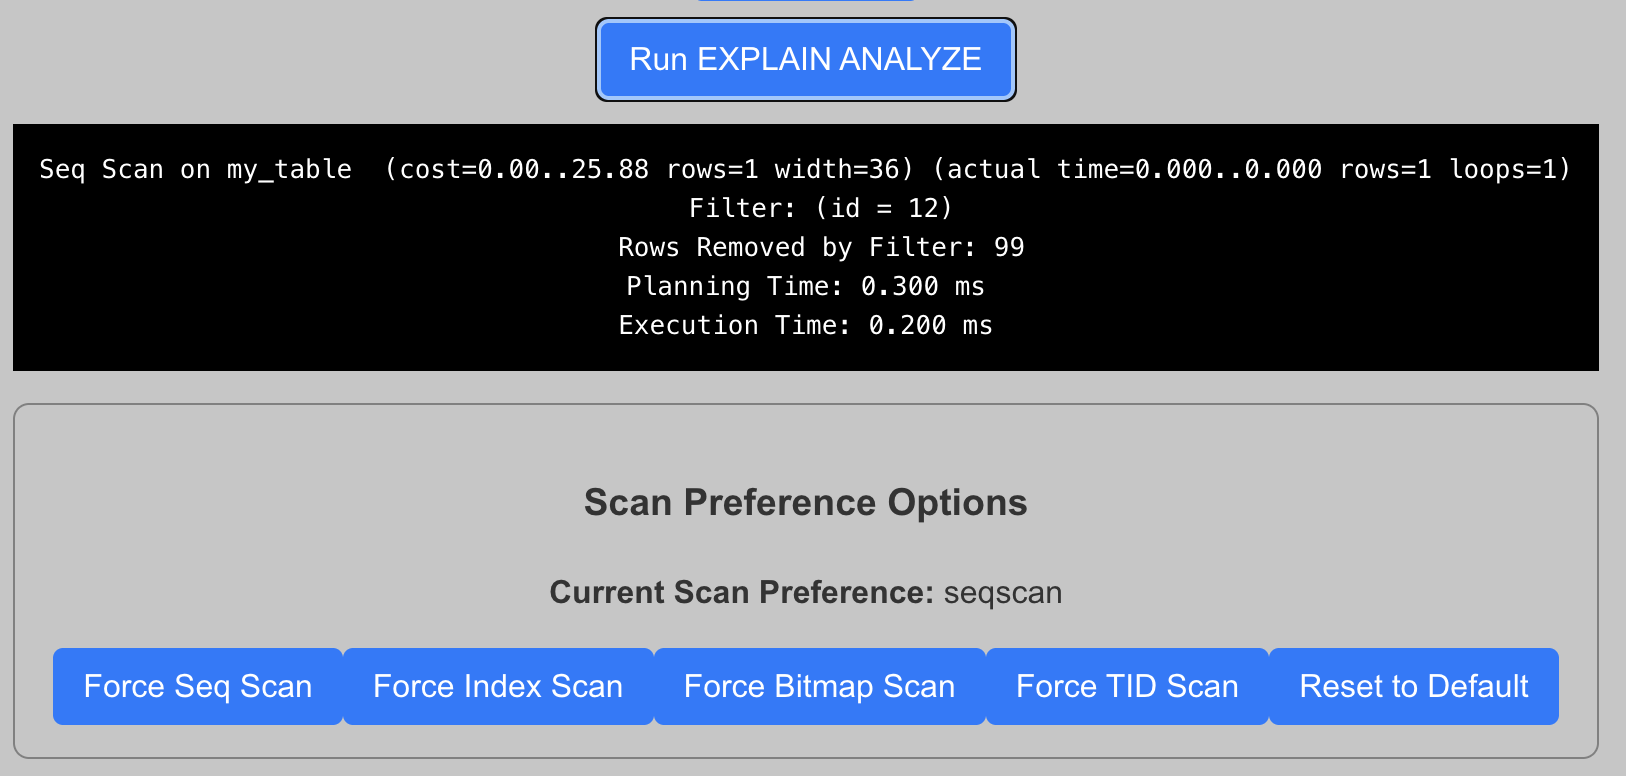
\includegraphics[width=0.8\textwidth]{seq.png}
    \caption{Selecting Sequential Scan for a query}
\end{figure}


\begin{figure}[htbp]
    \centering
    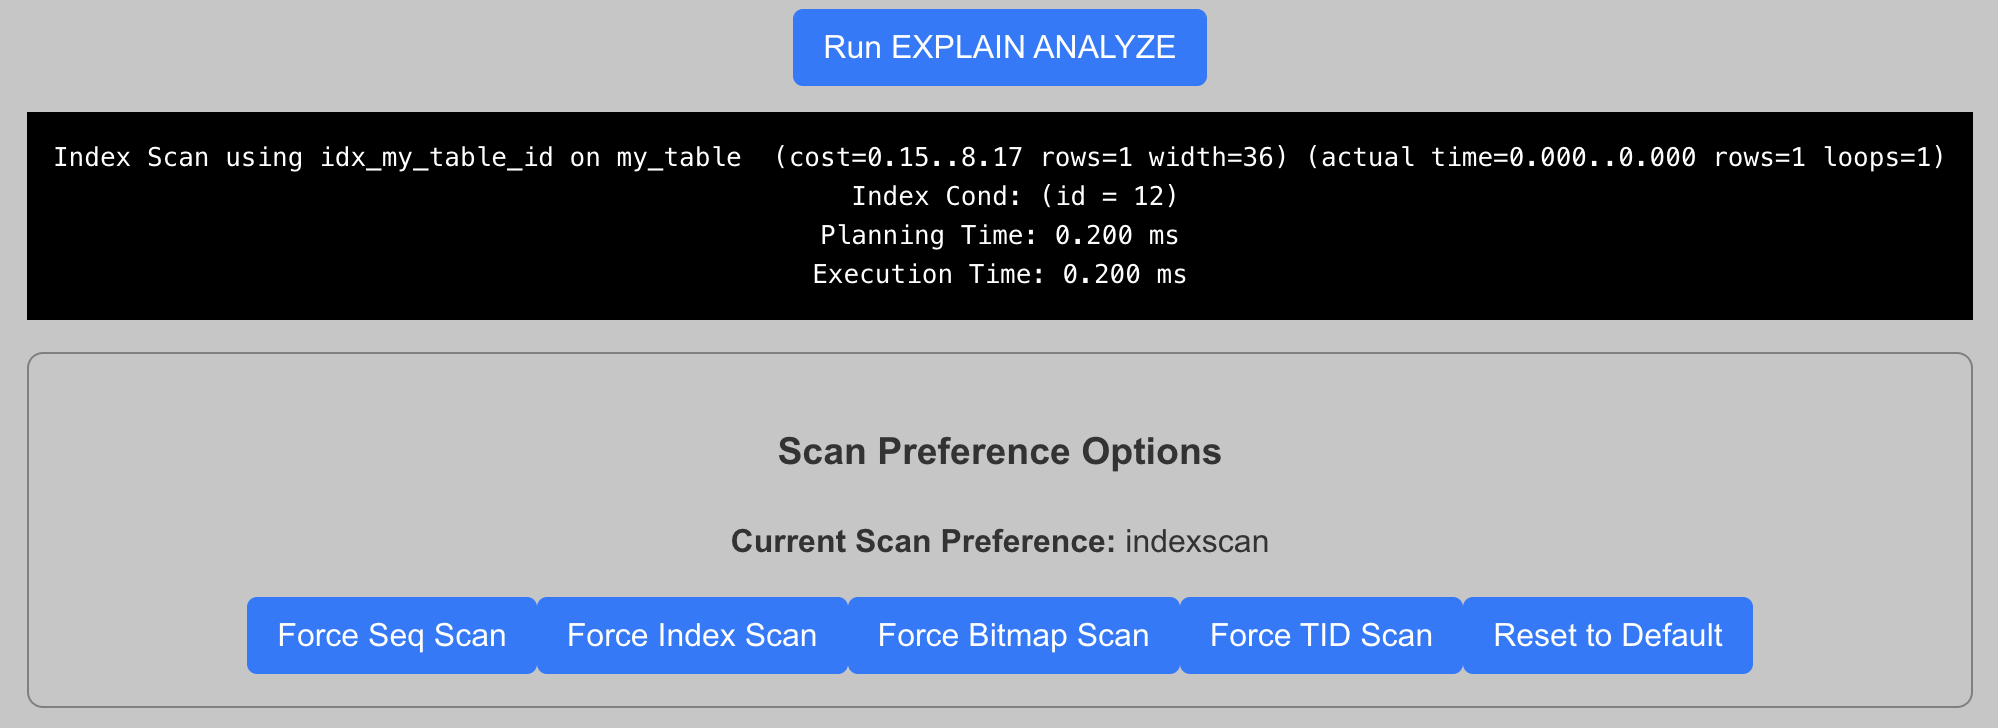
\includegraphics[width=0.8\textwidth]{index.png}
    \caption{Selecting Index Scan for a query}
\end{figure}

The main utility of this feature is that sometimes the query planner chooses a suboptimal evaluation plan for a query. This can happen if the statistics of the tables involved in the query are not up to date. In such cases, the user can look at the performance of different evaluation plans and choose the best one. This feature is useful for debugging and optimizing queries.


\subsection{Other Features}

The other 3 features are still being worked on. We have included them in our future plan of action and provided a rough timeline for their implementation.

\section{Future Plan of Action}

\section{Rough Timeline}

\section{Integration with XData Code}

\section{Challenges Faced}

\section{Conclusion}

    
\end{document}